\chapter{基于关系拓扑结构及描述文本的本体嵌入}
本体是领域内公认的概念的集合,是对一系列关系和实体的抽象描述,能够对目标域知识图谱中的未见关系和未见实体提供语义信息,实现零样本学习。为了能够从本体中学习到关系和实体的语义信息,以便将本体信息进行高效的表示学习并用于后续的知识图谱嵌入,需要在本体中补充与关系相关的三元组。本文通过提取实例知识图谱三元组中的关系头尾节点信息和关系间的拓扑信息,得到了关系的定义域、值域三元组以及关系位置元关系三元组,以此构建了关系加强的本体图。之后利用本体概念的描述文本信息对结构层面的本体嵌入进行增强,学习到了融合本体三元组结构信息和描述文本信息的本体嵌入。

\section{基于关系拓扑结构及描述文本的本体嵌入框架}
如图\ref{fig:new-3-1}所示,基于关系拓扑结构及描述文本的本体信息嵌入框架主要包含关系本体构建和基于描述文本的本体表示两个部分。作为本体嵌入的基础,本文了解到大多数引入本体信息的模型仅通过实体的类型和层次信息作为本体信息的体现,忽略了关系在本体中的体现。因此,本文首先对实例知识图谱中的关系进行处理,将关系的首尾实体抽象为实体类型,构建了关系的domain、range相关的本体三元组。考虑到知识图谱中关系的语义相关性,本文提出四种关系的位置元关系进一步对本体中的关系信息进行加强。而后在本体三元组的基础上学习对本体信息的嵌入。在通过传统KGE方法对本体三元组结构信息嵌入的基础上,本文又引入了本体节点的描述文本对本体嵌入的语义进行加强,获得了最终的本体向量表示。
\begin{figure}[h]
  \centering
  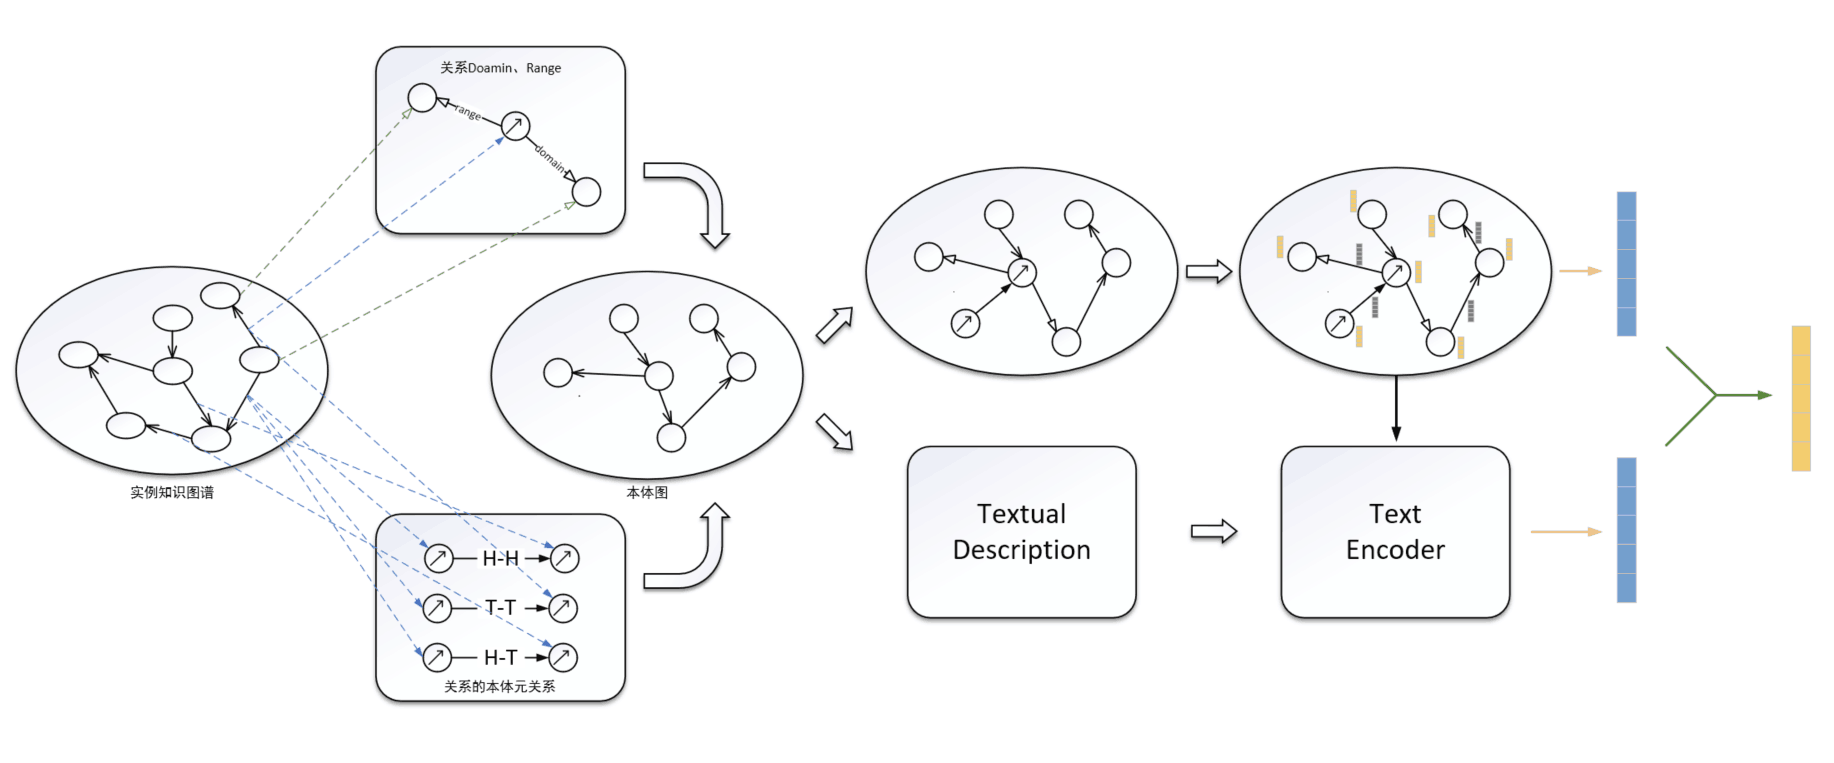
\includegraphics[width=1\textwidth]{new-3-1.png}
  \caption{本体嵌入整体框架}
  \label{fig:new-3-1}
\end{figure}

\section{关系本体图构建}
结合本体的知识表示模型往往仅使用了实体类型、层次等信息,忽略了关系在本体中的重要体现。本节将介绍本文如何在现有的本体三元组基础上,对关系相关的本体三元组进行补充。同时,根据关系的相对位置定义了四种关系的位置元关系,对本体中的关系信息进行加强。

\subsection{关系本体三元组}
在资源描述框架(Resource Description Framework,RDF)的设置下,知识图谱中的知识总是以三元组的形式出现,通过RDF的主语、谓语和宾语来描述事实。RDF通过类和属性描述个体之间的关系。这些类和属性由模式定义。RDF模式(RDF Schema,RDFS)提供了最基本的对类和属性的定义。其中,类有type和subClassOf两种定义,分别用于指定个体所属的类以及子类和父类之间的关系。对于属性,有三种核心属性,分别是subPropertyOf、domain和range,用于指定子属性与父属性之间的关系,以及属性适用范围和取值范围。

RDFS通过定义的方式来描述元数据之间的关系。同时,通过定义可以将知识分为两类:一类是数据层面的知识,如(Obama,type,Person)说明Obama是Person的一个实例;另一类是模式层面的知识,如(speaker,domain,Person)说明speaker属性的定义域是Person类。从简单意义上讲,数据层面的知识更多作用于实体,而模式层面的知识更多作用于关系。但当下将本体信息引入知识图谱嵌入的方法大多数仅采用数据层面的知识,忽略了模式层面知识对实例关系的知识补充。例如TransT\cite{ma2017transt}模型根据头尾实体的类型计算相似度,并作为知识图谱的先验知识改进三元组评分;JOIE\cite{hao2019universal}模型通过实体的本体类型信息将本体图和实例图进行跨视图的表示学习。这些模型主要通过本体的数据层面的知识,如实体类型对表示学习进行加强,更多偏向于实体的知识补充,忽略了对关系的补充。而跨域知识图谱中存在未见关系,本体中对关系模式的补充是非常必要的。
\begin{figure}[h]
  \centering
  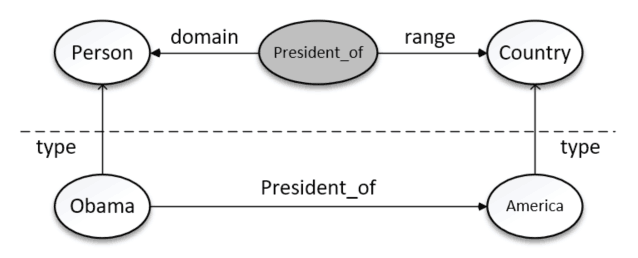
\includegraphics[width=0.6\textwidth]{new-3-2.png}
  \caption{关系本体三元组}
  \label{fig:3-2}
\end{figure}

同样借助于实体的类型,本文通过对实例图谱中事实三元组的处理提取关系的本体三元组。如图\ref{fig:3-2}所示,对一个事实三元组(Obama,President\_of,America),其中头尾实体的本体类型三元组为(Obama,type,Person)和(America,type,Country),可知对于关系President\_of在本体中的定义域即头本体应该是类型Person,值域即尾本体,因此构建出相应的关系本体三元组(President\_of,domain,Person)和(President\_of,range,country)。

但从源知识图谱直接抽取会产生大量的domain和range相关的关系本体三元组,其中包含了所有关系可能的值域和定义域。为了能够将抽取的关系的值域和定义域的本体三元组尽可能地表示最普适的元信息,对于抽取所有的关系本体三元组,本文通过统计关系本体三元组在实例知识图谱中出现的频率,设置阈值进行筛选,以出现频率来代表关系本体三元组的普适程度。除此之外,除了关系的domain和range的模式三元组,本文认为关系与关系之间存在相似性的关联,因此通过对关系描述文本的相似度匹配,计算关系与关系间的相似程度。本文将关系与关系的相似性关联及现有本体三元组中的isa、synonym元关系统一归类为generalizations元关系加入到本体三元组数据中。其中对关系描述文本的相似度匹配,本文采用word2vec进行文本嵌入和相似度计算。

\subsection{关系位置元关系}
关系本体三元组从值域和定义域的层面对本体中的关系信息进行了补充。除此之外,本文希望通过知识图谱中关系的语义相关性进一步对关系相关的语义信息进行捕捉。知识图谱中的实体具有隐含的语义相关性,例如北京和武汉在作为类型城市的实例中具有相似的语义。而关系的语义的相关性也非常常见,例如关系“/people/person/nationality”和“/people/ethnicity/languages\_spoken”具有很强的语义相关性,由于一个人说的语言很大程度上与他的国籍有关,在知识图谱上则可能直接表示为上述两个关系与同一个实体相关联。相反的,上述关系与语义差别很大的其他关系,如“/film/film/country”,则没有很强的语义相关性。并且这种语义相关性与关系的方向密切相关,如图\ref{fig:new-3-3}的“sister\_of”和通过e1节点连接的“has\_gender”,及通过e2节点连接的“sister\_gender”因为拓扑关系的不同,包含了完全不同的隐含信息。
\begin{figure}[h]
  \centering
  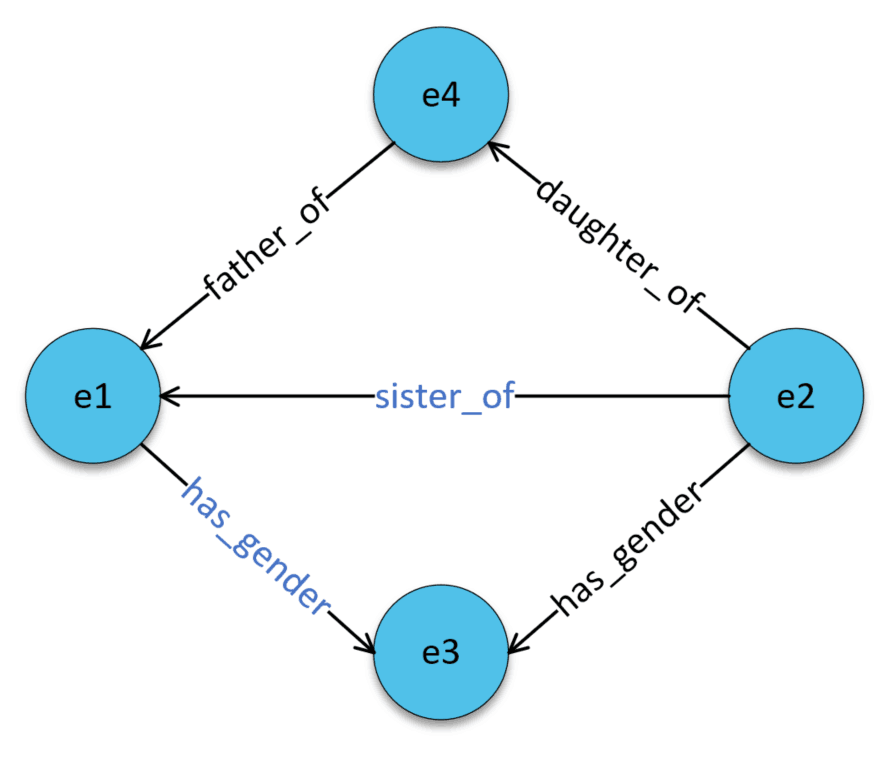
\includegraphics[width=0.4\textwidth]{new-3-3.png}
  \caption{关系位置实例}
  \label{fig:new-3-3}
\end{figure}

为了对两个关系之间的相关性进行建模,本文将关系与关系之间的拓扑关系建模为四种关系的位置元关系,如图\ref{fig:3-4}所示,分别为tail-head、head-tail、tail-tail、head-head。位置元关系的头结点和尾结点都代表了两个相邻关系的指向,比如(relation1,tail-head,relation2)代表同一个实体连接的两个相邻关系1和关系2,且关系1指向该实体而关系2则从该实体指向其他实体。对于训练三元组中的两个关系,如果它们符合其中一种的相对位置关系,则提取一个位置元关系补充到本体三元组中。
\begin{figure}[h]
  \centering
  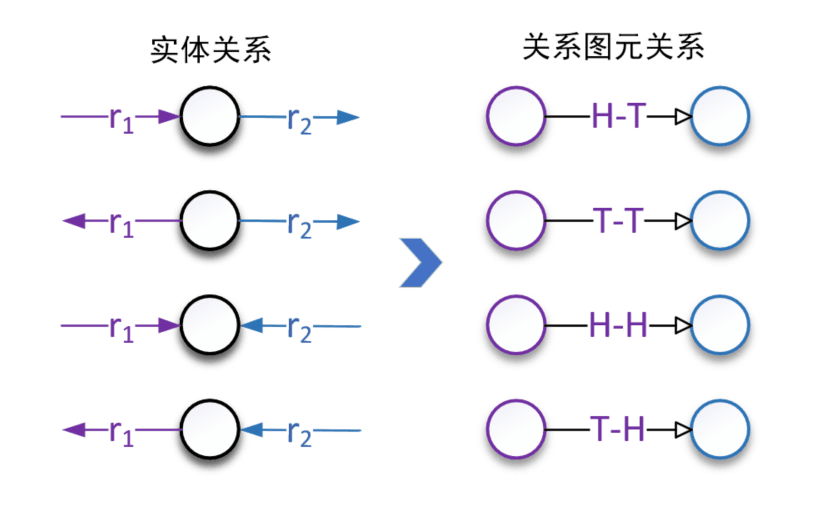
\includegraphics[width=0.6\textwidth]{3-4.png}
  \caption{实体关系与关系图元关系的映射}
  \label{fig:3-4}
\end{figure}

将位置元关系补充到本体三元组中后,本文希望通过传统的知识图谱嵌入方法对本体概念学习向量表示。但对位置元关系分析可知,“head-head”元关系自身、“tail-tail”元关系自身以及“head-tail”和“tail-head”元关系对都具有对称性。如图\ref{fig:new-3-3}中通过e1连接的“sister\_of”和“has\_gender”关系存在有(sister\_of,head-tail,has\_gender)与(has\_gender,tail-head,sister\_of),通过本文第2章对On2Vec模型的分析可知无法采用传统的KGE方法对有对称的元关系直接进行嵌入。因此,本文在补充位置元关系时仅保留了“head-tail”、“head-head”和“tail-tail”元关系,并对“head-head”、“tail-tail”进行去重,避免了具有对称性位置元关系的存在。

通过对上述两种关系本体信息的补充,结合实体类型相关的本体三元组,本文在本体三元组中保留了domain、range、generalizations以及三个位置元关系总计6种元关系。本体三元组统计数据如表\ref{tab:3-1}所示,最终构建出的本体图局部如图\ref{fig:new-3-5}所示。
% \begin{table}[h]
%   \caption{本体三元组统计信息}
%   \label{tab:3-1}
%   \centering
%   \resizebox{0.7\textwidth}{!}{%
%   \begin{tabular}{ccccc}
%   \hline
%   {\color[HTML]{333333} }         & {\color[HTML]{333333} 关系三元组数} & {\color[HTML]{333333} 元关系三元组数} & {\color[HTML]{333333} 其他三元组} & {\color[HTML]{333333} 总计}   \\ \hline
%   {\color[HTML]{333333} NELL\_Ext} & {\color[HTML]{333333} 1816}   & {\color[HTML]{333333} 2135}    & {\color[HTML]{333333} 332}   & {\color[HTML]{333333} 4326} \\
%   {\color[HTML]{333333} DB\_Ext}   & {\color[HTML]{333333} 1727}   & {\color[HTML]{333333} 1104}    & {\color[HTML]{333333} 464}   & {\color[HTML]{333333} 3295} \\ \hline
%   \end{tabular}%
%   }
%   \end{table}
\begin{table}[h]
  \caption{本体三元组统计信息}
  \label{tab:3-1}
  \centering
  \resizebox{0.7\textwidth}{!}{%
  \begin{tabular}{@{}ccccc@{}}
  \toprule
  {\color[HTML]{333333} }         & {\color[HTML]{333333} \textbf{关系三元组数}} & {\color[HTML]{333333} \textbf{元关系三元组数}} & {\color[HTML]{333333} \textbf{其他三元组}} & {\color[HTML]{333333} \textbf{总计}} \\ \midrule
  {\color[HTML]{333333} NELL\_Ext} & {\color[HTML]{333333} 1816}            & {\color[HTML]{333333} 2135}             & {\color[HTML]{333333} 332}            & {\color[HTML]{333333} 4326}        \\
  {\color[HTML]{333333} DB\_Ext}   & {\color[HTML]{333333} 1727}            & {\color[HTML]{333333} 1104}             & {\color[HTML]{333333} 464}            & {\color[HTML]{333333} 3295}        \\ \bottomrule
  \end{tabular}%
  }
  \end{table}
\begin{figure}[ht]
  \centering
  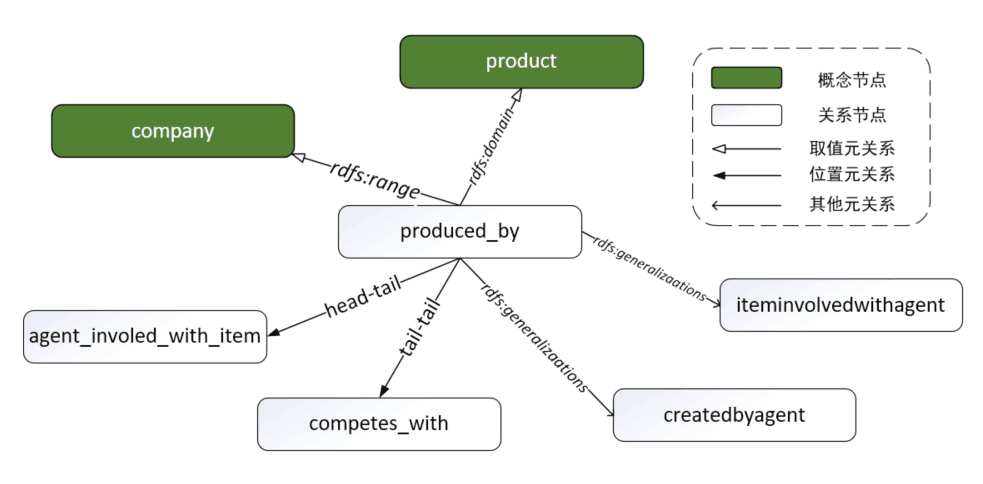
\includegraphics[width=0.8\textwidth]{new-3-5.png}
  \caption{关系本体图}
  \label{fig:new-3-5}
\end{figure}

\section{基于描述文本的本体表示增强}
\begin{figure}[!b]
  \centering
  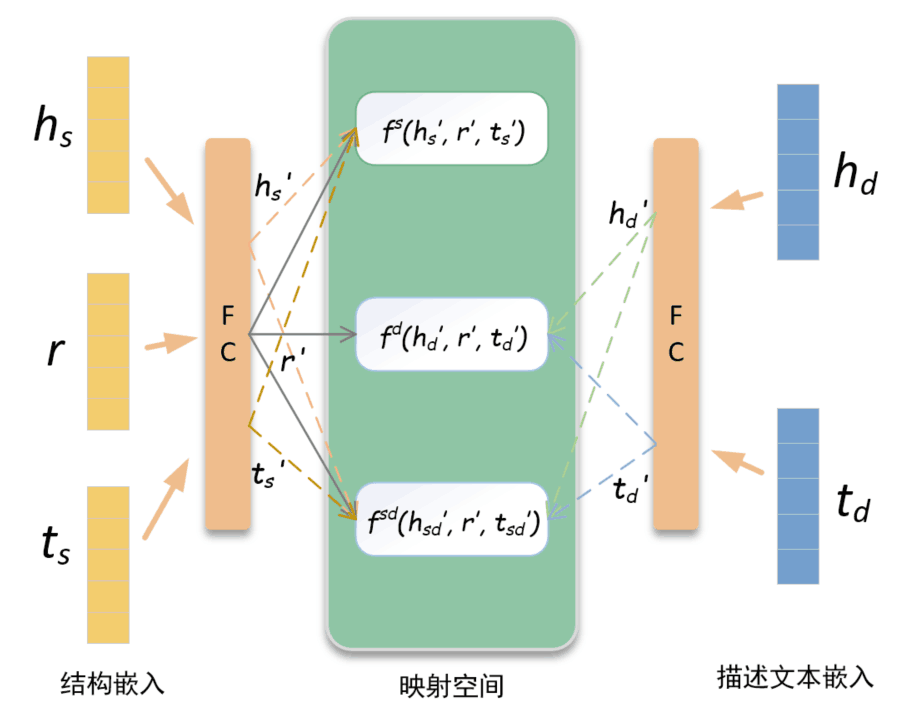
\includegraphics[width=0.7\textwidth]{3-2.png}
  \caption{本体嵌入架构}
  \label{fig:3-6}
\end{figure}

为了将符号化的本体三元组用于后续对未见实体和未见关系的语义补充,需要将本体三元组转化为低维向量表示。本节先从基础的本体三元组数据中学习到结构化的嵌入表示,然后从三元组的概念节点的描述信息中使用词嵌入学习到概念节点的描述文本嵌入。为了将描述文本的嵌入补充到本体信息的结构化表示中去,本文使用一个共享参数的线性层将结构化嵌入表示和描述文本嵌入表示映射到同一个表示空间中。在映射后的线性层中,参照TransE的评分方法,本文采用三个距离打分函数将映射后的两种嵌入表示联合更新,学习到兼顾结构信息和描述文本信息的嵌入表示。最后将两种表示拼接后作为本体信息进行后续操作。基于描述文本的本体表示增强结构图\ref{fig:3-6}所示。

\subsection{本体结构信息嵌入}
如前文所述,本文在构建本体三元组时降低了对称关系对嵌入效果的影响,因此可以应用多种传统的知识图谱嵌入方法学习本体表示。与传统的知识图谱嵌入表示类似,对于一个本体三元组\((c_{i},p,c_{j})\),本体语义信息编码的目的就是设计出一个打分函数\(f(c_{i},p,c_{j})\)作为编码模型的激活函数,本文采用RotatE对本体三元组进行编码。按照RotatE模型的设定,本体三元组的元关系属性是头尾两个实体节点的转移量,打分函数如公式\ref{eq:3-1}所示:
\begin{equation}
  f_{RotatE}(c_{i},p,c_{j}) = - \| \textbf{c}_{i} \circ \textbf{p} + \textbf{c}_{j}\|, \label{eq:3-1}
\end{equation}
其中\(\textbf{c}_{i}\),\(\textbf{p}\),\(\textbf{c}_{j}\)是一个本体三元组相应的概念编码和元关系编码,\(\circ\)指代了向量的旋转操作。同时为了提高所有本体三元组的嵌入效果,本文采用自对抗负抽样损失函数来计算损失并更新模型,如公式\ref{eq:3-2}所示:
\begin{equation}
  \mathcal{L}_{\mathcal{O}} = \frac{1}{\mid \mathcal{T}_{\mathcal{O}}\mid} \sum_{(c_{i},p,c_{j}) \in \mathcal{T}_{\mathcal{O}}} [\gamma _{o} + f(c'_{i},p,c'_{j}) + f(c_{i},p,c_{j})], \label{eq:3-2}
\end{equation}
其中\(\gamma _{o}\)是控制正负样本得分的参数,\(c_{i}\),\(c_{j}\)是不存在于本体三元组中的负样本。为了生成这些负样本,本文在所有的本体概念中分别遮盖住已存在的本体三元组的头节点和尾结点,然后从所有本体节点中随机筛选出其他节点组成负样本。

\subsection{基于文本的本体嵌入}
除了结构化的本体三元组外,本体信息还有许多对本体进行详细描述的文本,如本体概念“companyceo”的描述文本“specifies that a particular CEO is the CEO of a particular company”。这些描述文本可以为本体信息提取提供额外的语义信息,因此本文通过使用文本描述来加强对本体三元组的语义嵌入。然而,描述文本的建模与一般的三元组建模因模型的差异而无法直接融合。因此对于给定的本体三元组\((c_{i},p,c_{j})\),本文首先获得了三元组的结构嵌入\(h_{s}/r/t_{s} \in \mathbb{R}^{d_{1}}\)和每个本体节点描述文本的向量表示\(h_{d}/t_{d} \in \mathbb{R}^{d_{2}}\),表示文本描述信息。为了融合这两个不同层面的嵌入,本文引入了一个全连接层,将两个不同的嵌入映射到同一表示维度上。映射后的结构嵌入和文本嵌入分别表示为\(h_{s}^{'}\)和\(h_{d}^{'}\),在统一表示空间中,使用TransE对三元组结构的嵌入进行打分,打分函数如公式\ref{eq:3-3}所示:
\begin{equation}
  f^{s} = -  \parallel h'_{s} + r' - t'_{s}  \parallel, \label{eq:3-3}
\end{equation}

对描述文本的嵌入进行打分,打分函数如公式\ref{eq:3-4}所示:
\begin{equation}
  f^{d} = -  \parallel h'_{d} + r' - t'_{d}  \parallel, \label{eq:3-4}
\end{equation}

同时为了使这两种类型的表示相互兼容和互补,本文遵循DKRL模型的设定来定义交叉和相加得分函数,打分函数如公式\ref{eq:3-5}所示:
\begin{equation}
  f^{sd} = -  \parallel h'_{s} + r' - t'_{d}  \parallel -  \parallel h'_{d} + r' - t'_{s}  \parallel, \label{eq:3-5}
\end{equation}

三个得分函数的综合可以保证两个层面的嵌入表示可以在相同空间里进行学习和更新,最后本体嵌入的得分函数如公式\ref{eq:3-6}所示:
\begin{equation}
  f'(c_{i},p,c_{j}) = f^{s} + f^{d} +f^{sd}, \label{eq:3-6}
\end{equation}

从而在本体嵌入的损失函数也相应的转化为公式\ref{eq:3-7}:
\begin{equation}
  \mathcal{L}_{\mathcal{O}}^{ont} = \frac{1}{\mid \mathcal{T}_{\mathcal{O}}\mid} \sum_{(c_{i},p,c_{j}) \in \mathcal{T}_{\mathcal{O}}} [\gamma _{o} + f'(c'_{i},p,c'_{j}) + f'(c_{i},p,c_{j})], \label{eq:3-7}
\end{equation}

经过训练后每个本体节点都有两个层面的嵌入:三元组结构嵌入和描述文本嵌入。本文将这两种映射后的嵌入进行拼接作为本体节点的最终向量表示。上述描述文本的向量表示,本文采用了词袋模型进行生成。

\section{本章小结}
本章通过对本体三元组的关系部分构建,强调了关系在本体信息中的体现。尤其是在处理跨域知识图谱中存在的新的关系,本体中的信息能够对关系表示进行有效的语义补充。通过本体三元组的结构信息和本体的描述文本信息,能够学习到好的本体嵌入,为下一章未见关系的建模提供了良好的先验知识。